%\documentclass{article}
%\usepackage{algorithm2e}
%\begin{document}
\section{Route Planning}
\label{Imp:sec:routePlanning}
Planning an agent's route from its current point to a given point is acheived by a collaboration between a Person and PersonNavmeshRoutePlanner instance. Routes are stored using the jMonkeyEngine class MotionPath. This contains a set of waypoints and methods to animate the agent's movement between these waypoints. The maximum distance between each waypoint is roughly constant and can be set as a parameter to the following procedure (it is not constant when the agent must turn at a point closer to its current position that the maximum distance between points). The distance used is an important decision in the implementation. If it is too large the accuracy of the animation tends to degrade. If it is too low then a large number of waypoints will be stored needlessly. After extensive experimentation 0.5 was found to be an acceptable value for the maximum distance between waypoints. In practice this provided a balance between quality and efficiency.\\
A route is calculated in two stages:
\begin{enumerate}
\item{A path is calculated on the navigation mesh using a modified A* algorithm to traverse the mesh like a graph. This returns a small set of points. These points illustrate the lines of motion an agent must take to reach their goal. This is performed in the constructor for a PersonNavmeshRoutePlanner.}
\item{Using these points as guidance, the path is `fleshed out' by moving along the path and placing MotionPath waypoints no further apart than the defined maximum
distance. This terminates with a waypoint being placed on the goal location the agent must reach.}
\end{enumerate}
Note that a fresh PersonNavmeshRoutePlanner instance must be instantiated to calculate a route. The relationship between the Person and PersonNavmeshRoutePlanner instances is expressed in \ref{fig:RoutePlanSequence}.

\begin{figure}
\label{fig:RoutePlanSequence}
\centering
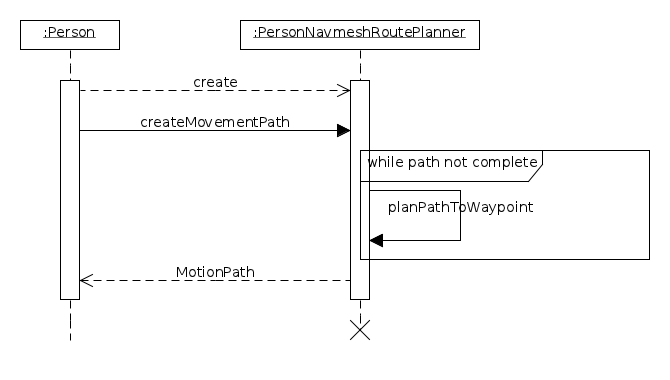
\includegraphics[scale=0.5]{../UMLDiagrams/RoutePlanningSequence.png}
\caption{Generation of an agent route as a MotionPath}
\end{figure}


\section{Implementing the Perceive, Decide, Act Process}
\label{Imp:sec:perceiveDecideAct}
Here we discuss the techniques and algorithms used to realise the Perceive, Decide, Act process previously discussed in Section \ref{Res:subsec:perceiveDecideAct}.

%%%%%%%%%%%%%%%%%%%%%%%%%Perception Implementation
\subsection{Perception}
\label{Imp:subsec:perception}
Agent perception is achieved using the following simple algorithm:

\begin{algorithm}[H] %%%%%%%Agent Perception Algorithms
 \SetAlgoLined
 \SetKwInOut{Input}{input}
 \SetKwInOut{Output}{output}
 \Input{The set of goals in the environment: \emph{goals}}
 \Output{A set of goals visible to the user at the given instant in time: \emph{visibleGoals}}
 \BlankLine
 \For{each goal g in goals}{
  \If{g is in line of sight of agent}{
    add g to visibleGoals\;
  }
  }
  \caption{Agent Perception Algorithm}
\end{algorithm}

%%%%%%%%%%%%%%%%%%%%%%%%%%%%%Decision Implementation
\subsection{Decision}
\label{Imp:subsec:decision}
In the Research Chapter [Reference] the three classes of human behaviour considered in the scope of this project were defined. In practice, only herding behaviour implemented as part of the Decide step; queueing and competetive behaviour must be handled asynchronously using collision avoidance techniques. Unfortunately collison avoidance was not implemented in the final system due to various problems discussed in Section \ref{Problems:subsec:problemsecountered}. Future solutions to implement collision avoidance are discussed in Section \ref{Problems:subsubsec:ORCA}.
To decide on a new action, an agent must select one of the visible goals that were found in the Perceive step (if any). Otherwise it must continue on its current path. The decision making process is realised using an extendable algorithm, which sequentially considers sets of different classes of goal according to their priority. Exits have the highest priority.\\

The final algorithm only makes decisions regarding exits, due to various issues which emerged during development (see Section \ref{Problems:subsec:problemsecountered}). However it is easy to extend this process to include other goal types by adding further conditionals following the pattern laid out below.\\

%%%%%%%%%%%%%%%%%%%%%%%%%%%Decide Algorithm
\begin{algorithm}[H]
 \SetAlgoLined
 \SetKwInOut{Input}{input}
 \SetKwInOut{Output}{output}
 \Input{Person person, ExitGoal[ ] exits /*add further exit types here as arrays */}
 \Output{Target Goal for agent to move toward}
 \eIf{no of exits $>$ 0}{
   ExitGoal \emph{currentExit} = $exits[0]$\;
   \eIf{person is stressed}{
     \For{each exit \emph{e} in exits}{
       \If{number of people queuing at e $>$ no. of people queueing at targetExit}{
	targetExit = e\;
	}
      }
    return targetExit\;
    }{ %%%%%%%%%%%inner else
     Vector3f position = person.location\;
     \For{each exit e in exits}{
       \If{distance to e $<$ distance to targetExit}{
	targetExit = e\;
	}
      }
      return targetExit\;
     }
}{ %%%%%%%%outer else
  return null;
}
\end{algorithm}

\subsection{Act}
\label{Imp:subsec:act}
This step's representation in the BehaviouralModel class is trivial since the Decide step already returns a target goal. It is left in as a place for performing any calculations which should be performed before returning the target goal to the agent.\\
Upon receiving a new target goal, an agent should perform the following:
\begin{itemize}
\item{Use a PersonNavmeshRoutePlanner to calculate a route to this goal}
\item{Set the returned MotionPath as the current MotionPath for the agent}
\item{Begin moving down this path}
\end{itemize}




%\end{document}
     
     
 

    

